%! Author = mboehme
%! Date = 01.03.2023

\newpage
\section{Ergebnis}\label{sec:ergebnis}
Abgleich der Ergebnisse mit den Soll-Anforderungen.
\subsection{Visuelle Darstellung}\label{subsec:visuelle-darstellung}
%include two images
\par\vspace{1cm}
\begin{figure}[h]
    \centering
    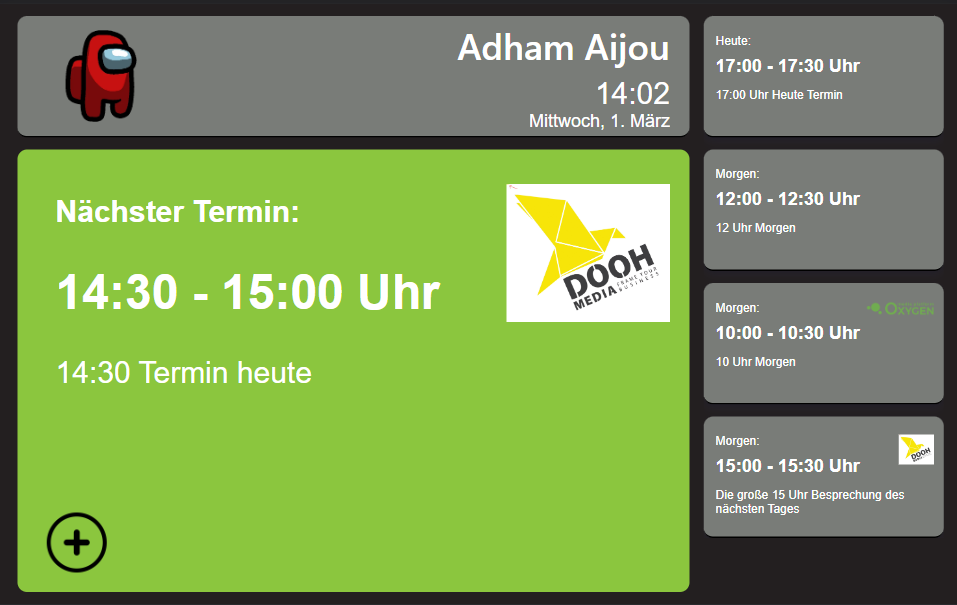
\includegraphics[width=0.8\textwidth]{Bilder/Ergebnis}
    \caption{Ergebnis mit nächstem anstehenden Termin}
    \label{fig:Ergebnis mit nächstem anstehenden Termin}
\par\vspace{1cm}
\end{figure}
\justifying
\par\vspace{1cm}
\begin{figure}[h]
    \centering
    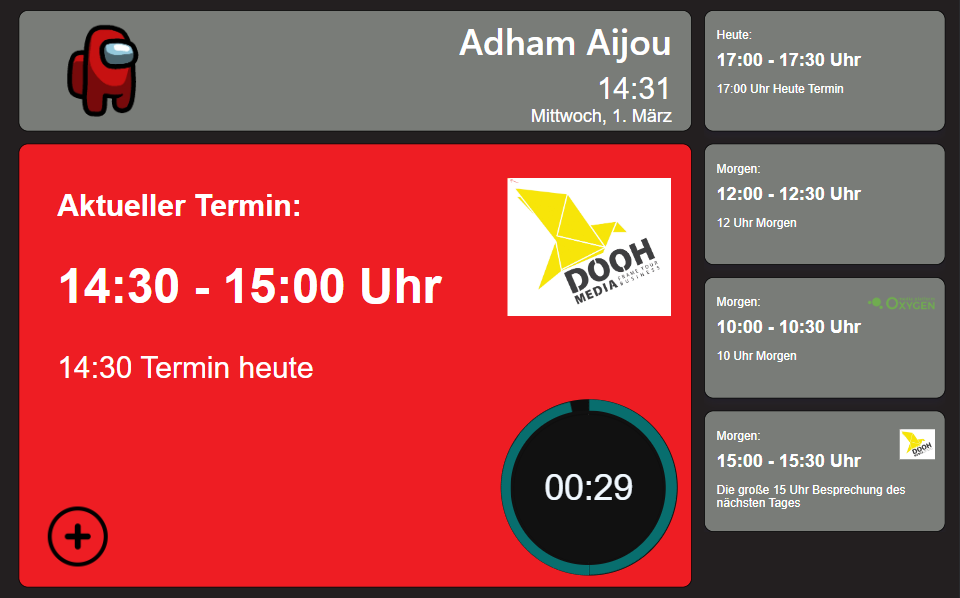
\includegraphics[width=0.8\textwidth]{Bilder/Ergebnis_LaufenderTermin}
    \caption{Ergebnis mit laufendem Termin}
    \label{fig:Ergebnis mit laufendem Termin}
\par\vspace{1cm}
\end{figure}
\justifying
\newline
Oben links im Bild, ist das Logo des Gastgebers des nächsten, beziehungsweise jetzigen, Termins zu sehen.
In diesem Fall ist dies das Logo der DOOH media GmbH\@.
Solch ein Logo kann dargestellt werden, indem beim Erstellen des Termins, außerhalb des Tablets, bei Outlook beispielsweise, ein Bild an den Termin angehangen wird, welches im Dateinamen \("\)Termin\_Logo\("\) enthält.
\newline
Die anderen Logos sind alle Logos vom Gast des Termins.
Sie werden angezeigt, indem der Firmenname im Textkörper des Termins vorkommt.
Um diese Logos initial den Firmennamen zuzuordnen, muss ein spezieller Termin erstellt wird, der nur für die Logos gedacht ist und eine einzigarte ID, sowie einen Befehl enthält, die dann das Bild, inklusive Firmennamen, in einer lokalen Datenbank abspeichert.
Diese Logos können hinzugefügt, gelöscht oder aktualisiert werden.
\newline
Die Uhrzeit wird immer in der Zeitzone des Tablets angezeigt.
\newline
\newline
%Das gehört in sollzustand.
Hier sieht man das Menü, in welchem ein Termin gebucht werden kann, welches durch das Drücken des Plus-Symbols aufgerufen wird:
\begin{figure}[h]
\par\vspace{1cm}
    \centering
    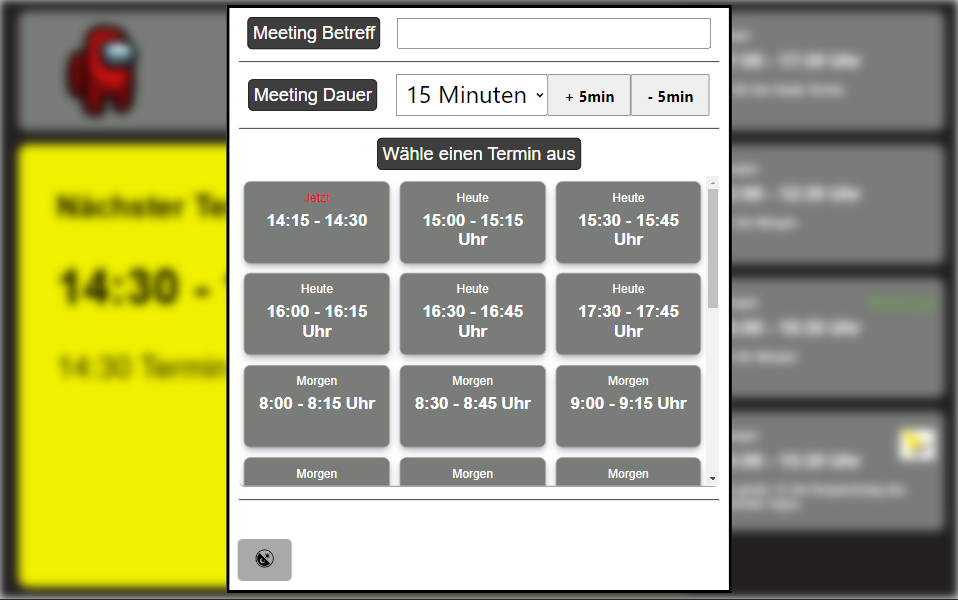
\includegraphics[width=0.8\textwidth]{Bilder/Ergebnis_TerminErstellen_Menue}
    \caption{Terminbuchungsmenü}
    \label{fig:Menue}
\par\vspace{1cm}
\end{figure}
\justifying
Wie zu sehen ist, ist beispielsweise die selbsterstellte Option \("\)Jetzt\("\) deaktiviert, da das Ende des hypothetischen Termins innerhalb von 15 Minuten vom nächsten anstehenden Termin beginnt.
Es werden alle möglichen Termine, innerhalb der Arbeitszeiten, für den Jetzigen und nächsten Tag angezeigt.
Falls z.B. der nächste Tag ein Feiertag ist, werden für den nächsten Tag keine Termine angezeigt.
Auf die anderen Optionen, wie z.B. Pufferzeiten, hat ein Anwender hier wenig Einfluss, da sie von den Einstellungen des Kalenders, des jeweiligen Nutzers, abhängen und es somit in der Verantwortung des Administrators liegt, diese zu ändern.
\newline
\newline
Hier die normale Ansicht nochmal, im hellen Design:
\par\vspace{1cm}
\begin{figure}[h]
    \centering
    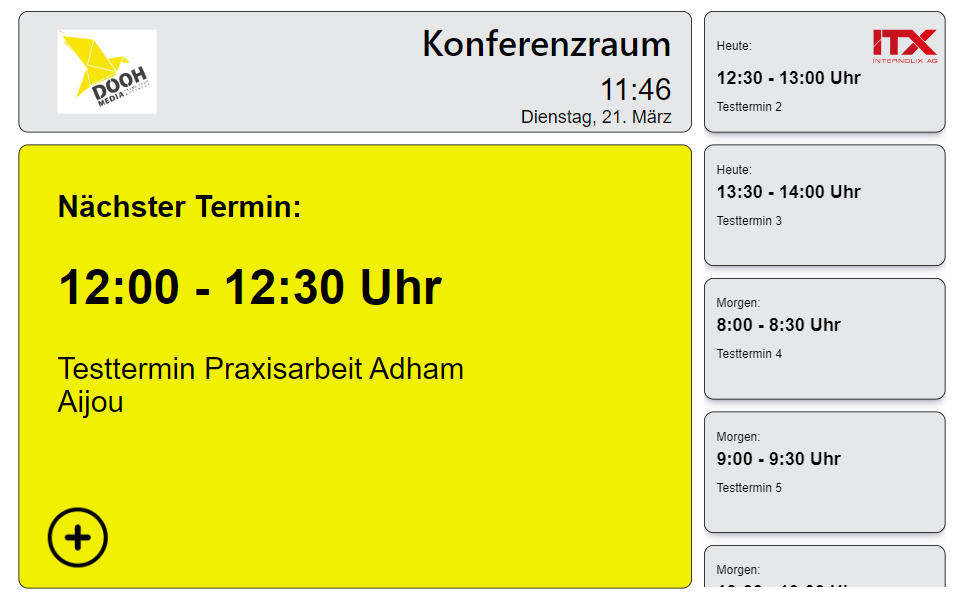
\includegraphics[width=0.8\textwidth]{Bilder/Ergebnis_lightMode}
    \caption{Ergebnis im hellen Design}
    \label{fig:Ergebnis im hellen Design}
\par\vspace{1cm}
\end{figure}
\justifying
\newline
\newline
\pagebreak
%Eigenes Kapitel
\subsection{Funktionalität}\label{subsec:funktionalitaet}
Alle Funktionalitäten aus den Soll-Anforderungen wurden umgesetzt.
\newline
Terminbuchungen, Synchronisation und LED-Strip Steuerung funktionieren wie in den Soll-Anforderungen beschrieben.
Um zu sehen, wie der Belegungsstatus eines Konferenzraums derzeit ist, muss also nicht ein Mal auf den Bildschirm geschaut werden, sondern es reicht, wenn man die LED Streifen aus der Ferne erkennt.
\newline
\newline
\subsection{Performance}\label{subsec:performance}
Die Performance einer \gls{SPA} zu messen ist trotz der geringen Komplexität der Anwendung, nicht simpel.
Auch die gängige Total-Blocking-Time Messung ist nicht zwingend sinnvoll, da die Anwendung nicht für den Nutzer, während der Nutzung, blockiert ist, sondern lediglich die Daten vom Server geladen werden, um anschließend die Nutzung der Anwendung sinnvoll zu ermöglichen.
\newglossaryentry{RAIL Modell}{name={RAIL Modell},description={Das RAIL Modell ist ein Modell, welches die Performance von Webseiten beschreibt. Es beschreibt, dass eine Webseite in 5 Bereiche unterteilt werden kann, welche die Performance beeinflussen. Diese sind: Antwort, Animation, Leerlauf, Laden und Bilder pro Sekunde.}}
Daher wurden manuell einige Tests durchgeführt, um die Performance zu messen und in Zusammenhang mit dem RAIL Modell~\cite{RAILModell} bewertet.
Es sollte dafür berücksichtigt werden, dass der Prozessor des Tablets, welches die Anwendung verwendet, ein 32 Bit Prozessor ist, welcher im Jahr 2013 auf den Markt kam.
\newline
\newline
%Tests brauchen Namen
\subsubsection{Initiales Laden}\Label{subsubsec:initiales-laden}
\newline
\newline
Die~\gls{TBT} der Applikation liegt, aufgrund von hoher Komplexität, bei ca. 500ms.
Somit ist das Laden der Webseite akzeptabel~\cite{TotalBlockingTime}, da die Total-Blocking-Time nicht die Grenze von 600ms überschreitet.
Das RAIL Modell erlaubt sogar Ladezeiten von bis zu 5 Sekunden beim initialen Laden der Webseite, falls innerhalb dieser 5 Sekunden die Interaktivität mit der Webseite gegeben ist.
Die Hardware, die hier verwendet wurde, besitzt einen 32 Bit Prozessor, welcher im Jahr 2013 auf den Markt kam.
\newline
\subsubsection{Test 1}\label{subsubsec:test-1}
\newline
\newline
Wie lange braucht die Anwendung, um nach einem Klick auf den Button \("\)+\("\) das Terminerstellungs-Menü zu öffnen?
\gls{Event-Listener}{name={Event-Listener},description={Ein Event-Listener ist ein Objekt, welches auf bestimmte Ereignisse wartet und dann eine Funktion ausführt. Dieses Objekt braucht ein HTML Element, welches es überwachen soll.}}
Die Antwort auf diese Fragestellung wurde gemessen, indem der Event-Listener für den Button \("\)+\("\) registriert ausgab, wann die Taste betätigt und damit Zeit gemessen wurde, die vergeht, bis der \gls{Event-Listener} das Menü darstellt.
Es dauert im Durchschnitt 2ms, bis das Menü angezeigt wird.
Damit sind wir weit unter der 100ms Grenze, welche das RAIL Modell für Interaktivität mindestens empfiehlt und weit unter den 50ms, welche das RAIL Modell anstrebt.
\newline
\newline
\subsubsection{Test 2}\label{subsubsec:test-2}
\newline
\newline
Wie viele Bilder pro Sekunde zeigt die Anwendung durchschnittlich an?
\newglossaryentry{LightHouse}{name={LightHouse},description={LightHouse ist ein Tool, welches von Google entwickelt wurde, um die Performance einer Website zu messen.}}
Dies wurde mithilfe von LightHouse gemessen.
%Aussage bewerten
Die Anwendung zeigt durchschnittlich 60 Bilder pro Sekunde an.
Da die maximale Wiederholrate des Bildschirms und des Browsers bei 60Hz liegen, besteht nicht die Möglichkeit, für diesen Anwendungsfall zu testen, ob noch mehr Bilder pro Sekunde angezeigt werden können.
Nichtsdestotrotz sind damit die Anforderungen des RAIL Modells für Bilder pro Sekunde erfüllt.
\newline
\newline
\subsubsection{Test 3}\label{subsubsec:test-3}
\newline
\newline
\newglossaryentry{Bottleneck}{name={Bottleneck},description={Der Bottleneck ist, in der Softwareentwicklung, die Stelle, an der die Leistung der gesamten Anwendung am meisten eingeschränkt wird.}}
Wie oft, kann die Anwendung theoretisch und praktisch pro Sekunde aktualisiert werden?
Für jede Kombination aus Azure App und E-Mail-Adresse, dürfen 10000 Anfragen pro 10 Minuten gemacht werden.
Dies sind 16,6 Anfragen pro Sekunde.
Praktisch wurden eine bis drei Anfragen, je nach Bedarf, pro drei Sekunden durchgeführt.
Dieser Bedarf hängt davon ab, ob sich an den Daten, die bei Microsoft gespeichert sind, etwas geändert hat und daran, ob Bilder-Anhänge für Gäste vorhanden sind, die nochmal separat per REST API abgefragt werden müssen.
Pro Sekunde wären das also 0,33 bis 1 Anfragen.
Einerseits ist das schnell genug für die Anwendung und gibt den langsamen Geräten, genug Zeit, die Anwendung zu aktualisieren, andererseits hat man so genug Anfragen übrig, falls jemand sein Konto mit mehreren Geräten benutzt oder dies in Kombinationen mit anderen Applikationen verwendet.
Sollte dieses Limit überschritten werden, verlangsamt Microsoft die Anzahl an neuen Antworten auf die Anfragen.
Da Microsoft auch Zeit benötigt, um die Anfragen zu bearbeiten und die neuen Daten bei sich zu verarbeiten, würde der Anwender den Unterschied selten bemerken.
Der \gls{Bottleneck} der Anwendung ist also in diesem Fall die Anzahl an Anfragen, die Microsoft, in ihren Servern, verarbeiten kann.
\newline
\newline
\subsection{Fazit}\label{subsec:fazit}
Die Microsoft Graph API ist eine sehr mächtige Schnittstelle, die es ermöglicht, mit einer Vielzahl an Microsoft Diensten zu interagieren.
Für die Anwendung wurde die Schnittstelle genutzt, um Termine zu erstellen, zu löschen und zu aktualisieren.
Außerdem wurde die Schnittstelle genutzt, um die Logos der anderen Termine zu erhalten.
Die Schnittstelle wurde nicht vollständig genutzt, da die Anwendung nicht alle Funktionen benötigt, aber bietet für die Zukunft viele Erweiterungsmöglichkeiten.
Zudem ist die API neu und wird ständig weiterentwickelt~\cite{microsoft-graph-api-version}.
Die Anwendung wurde mit der Version 1.0 der API entwickelt.
Für den Anwendungsfall des Kunden ist die API ausreichend, da die Anwendung nur Termine erstellen, löschen und aktualisieren muss.
Der einzige Nachteil ist, dass Azure AD, die Authentifizierung, für Ressourcenkonten nicht unterstützt, die beispielsweise, in Teams, genutzt werden.
Daher muss der Anwender sich mit einem Microsoft-Konto anmelden, welcher die Ressource repräsentieren soll.
Dies kann zu Verwirrung führen, da die Terminologie impliziert, man könne sich mit einem Ressourcenkonto anmelden.
\newline
\newline
Die API war die richtige Wahl für diesen Kundenauftrag.
Ressourcen- und Terminplanung wurde mit der Anwendung vereinfacht.
Ein Anwender braucht nur noch drei Klicks, um einen Termin zu erstellen und muss nicht mehr zwischen verschiedenen Kalendern hin und her wechseln.
%Aua, Fixen, umformen
Zudem benötigt ein Anwender lediglich einen Blick, um zu sehen, wann die Ressource, die durch die Software repräsentiert wird, frei ist und wann der Anwender gegebenenfalls einen Termin besitzt (Anhand der Logos).
\newline
\newline
Die Anwendung kann auch für menschliche Ressourcen genutzt werden, da die Anwendung keine Unterscheidung zwischen menschlichen und nicht-menschlichen Ressourcen macht.
Solche Entscheidungen obliegen dem Anwender.
\newline
\newline
Zusammenfassend kann gesagt werden, dass die Anwendung eine gute Basis für weitere Erweiterungen ist und die Anforderungen des Kunden so erfüllt.
Damit geht einher, dass die Ziele erreicht wurden.
\pagebreak
\newline
Abschließend folgt noch ein Bild des Gerätes mit der Anwendung, welches im Kundenbetrieb genutzt wird.
\newline
%Überleg dir was Anderes. Das ist hässlich.
%\par\vspace{1cm}
%\begin{figure}[h]
%    \centering
%    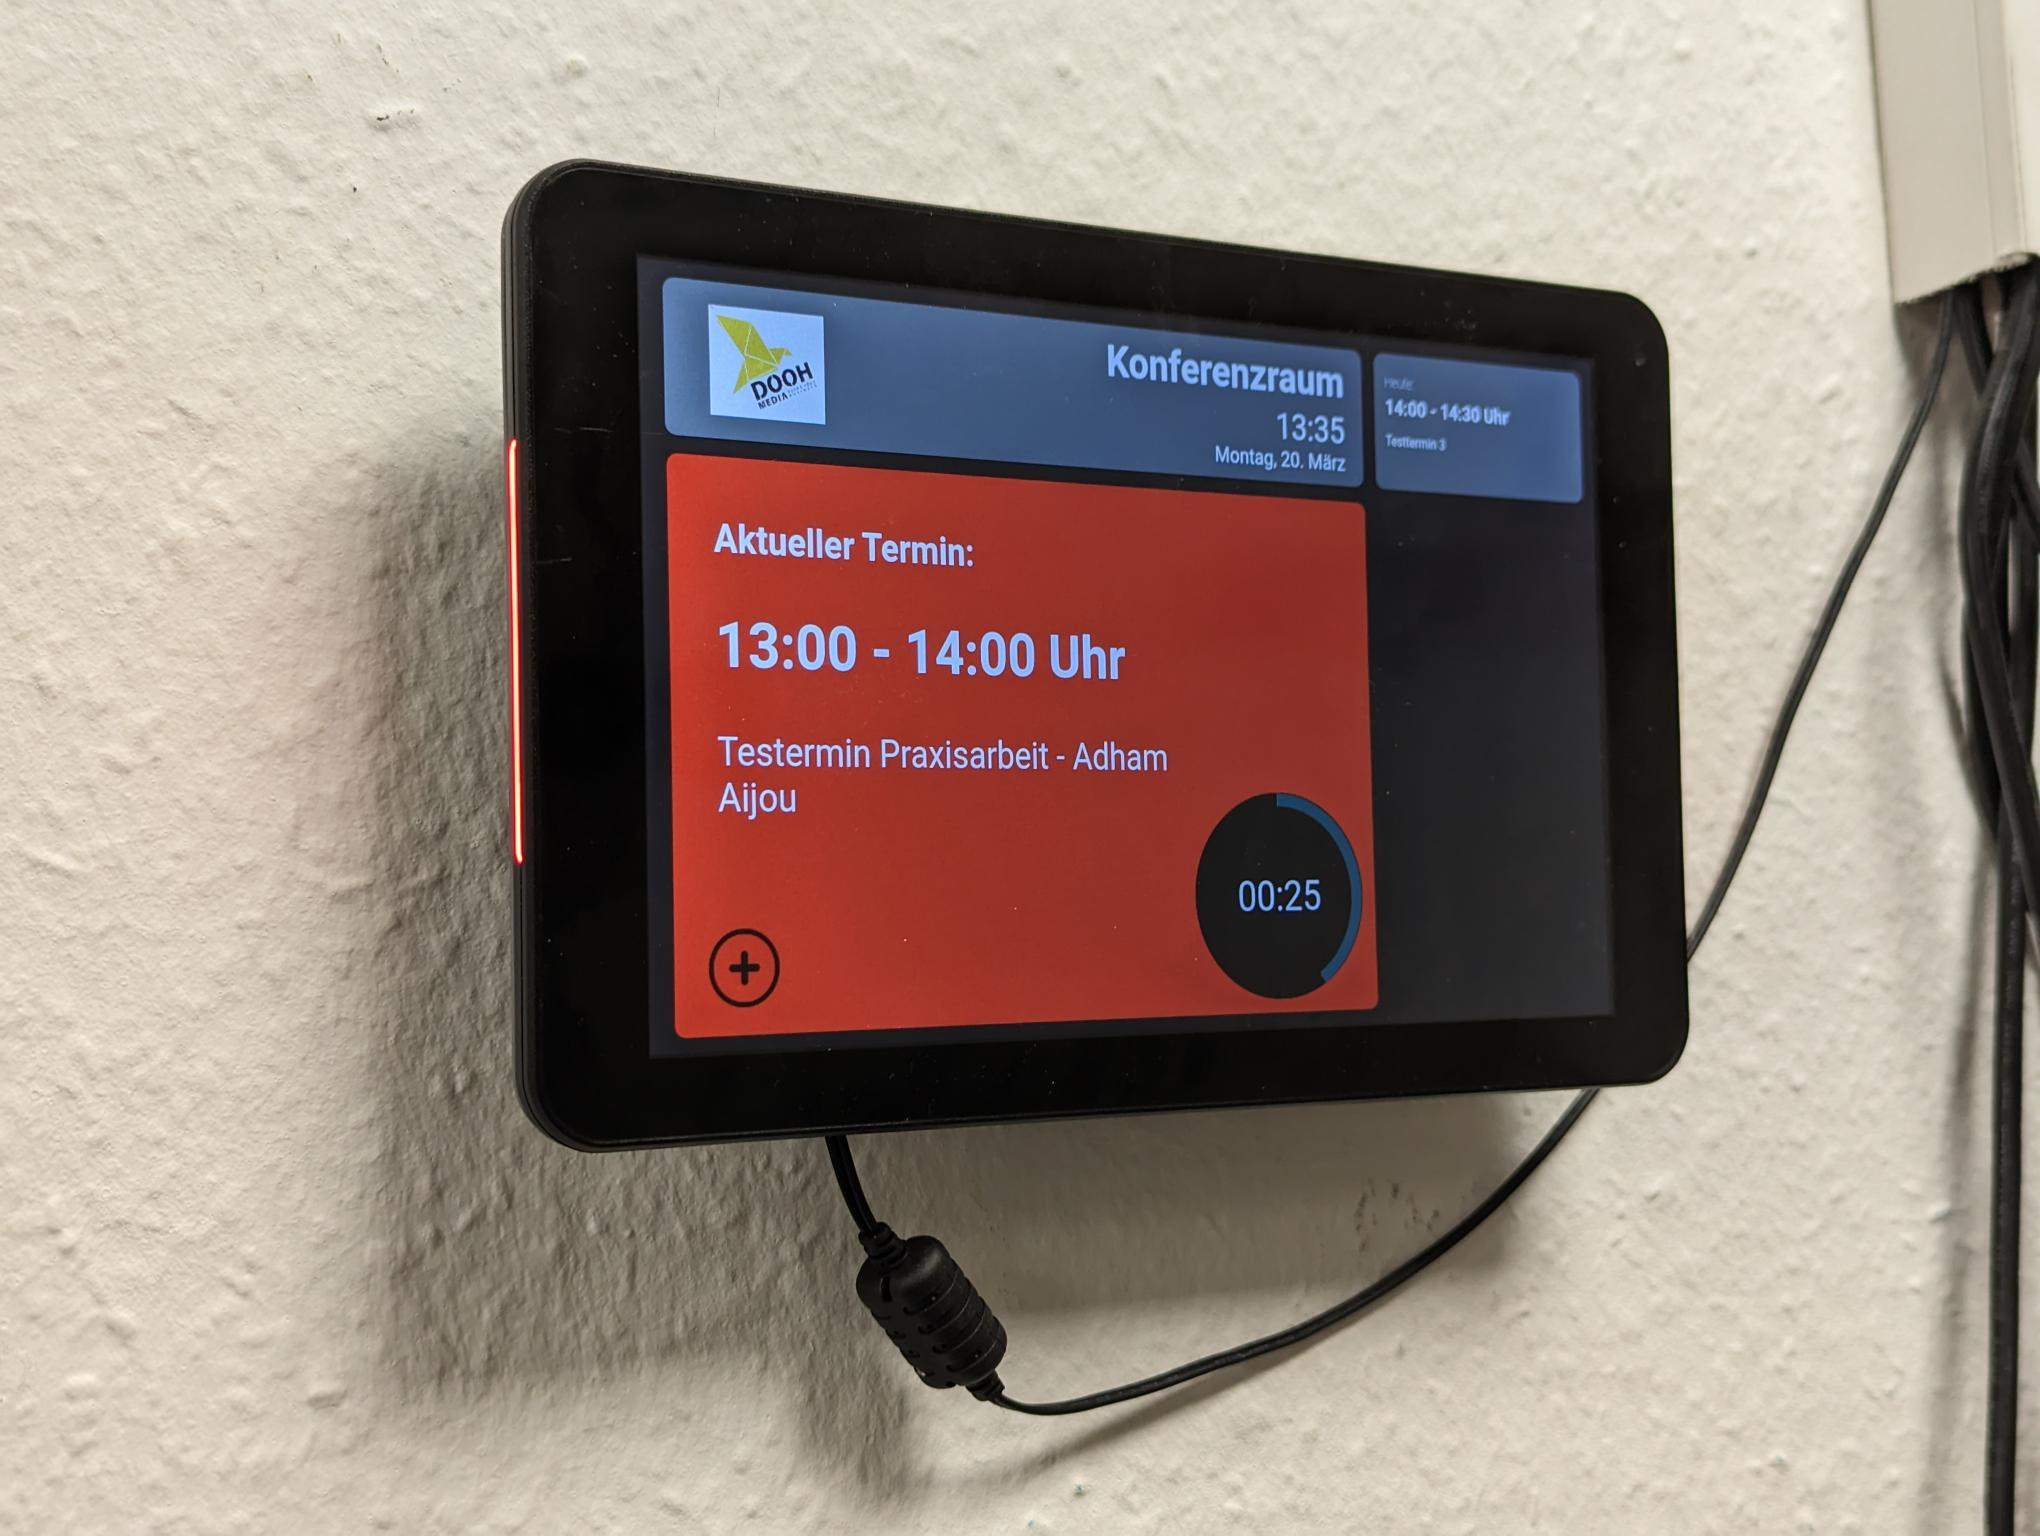
\includegraphics[width=0.5\textwidth]{Bilder/FertigesProdukt}
%    \caption{Fertiges Produkt - Gerät mit der Anwendung}
%    \label{fig:fertiges-produkt}
%\newline
%\newline
%    \end{figure}
\justifying
\newpage
\section{Literaturverzeichnis}\label{sec:literaturverzeichnis}